\documentclass[9pt,twocolumn,twoside,]{pnas-new}

%% Some pieces required from the pandoc template
\providecommand{\tightlist}{%
  \setlength{\itemsep}{0pt}\setlength{\parskip}{0pt}}

% Use the lineno option to display guide line numbers if required.
% Note that the use of elements such as single-column equations
% may affect the guide line number alignment.


\usepackage[T1]{fontenc}
\usepackage[utf8]{inputenc}


\templatetype{pnasresearcharticle}  % Choose template

\title{The Nature and Origins of the Lexicon in Six-month-olds}

\author[a,1]{Elika Bergelson}
\author[b, c]{Richard Aslin}

  \affil[a]{Duke University, Psychology \& Neuroscience, 417 Chapel Drive, Durham,
NC, 27708}
  \affil[b]{University of Rochester, Brain \& Cognitive Sciences, Meliora Hall,
Rochester, NY, 14627}
  \affil[c]{Haskins Laboratories, 300 George Street, New Haven, CT, 06511}


% Please give the surname of the lead author for the running footer
\leadauthor{Bergelson}

% Please add here a significance statement to explain the relevance of your work
\significancestatement{Infants start understanding words at six months, when they also excel at
subtle speech-sound distinctions and simple multi-modal associations,
but don't yet talk, walk, or point. However, true word-learning requires
integrating the speech-stream with the world, and learning how words
interrelate. Using eyetracking, we show that neophyte word learners
already represent the semantic relations between words. We further show
that these same infants' word learning has ties to their environment:
the more they hear labels for what they're looking at and attending to,
the stronger their overall comprehension. These results provide a new
integrative approach for investigating home-environment effects on early
language, and suggest that language delays could be detected in early
infancy for possible remediation.}


\authorcontributions{EB and RA developed the home-lab approach. EB and her staff conducted
eyetracking and home data collection. EB performed data analysis and
drafted the manuscript; RA provided feedback. Both approved the final
submitted version.}



\correspondingauthor{\textsuperscript{} }

% Keywords are not mandatory, but authors are strongly encouraged to provide them. If provided, please include two to five keywords, separated by the pipe symbol, e.g:
 \keywords{  Word Learning |  Lexicon |  Cognitive Development |  Language Acquisition |  Environmental Effects   }

\begin{abstract}
Recent research reported the surprising finding that even six-month-olds
understand common nouns (Bergelson \& Swingley, 2012 PNAS, 109,
3253-3258). But is their early lexicon structured and acquired like
older learners'? We test six-month-olds for a hallmark of the mature
lexicon: cross-word relations. We also examine whether properties of the
home environment that have been linked with lexical knowledge in older
children are detectable in the initial stage of comprehension. We use a
new dataset, which includes in-lab comprehension and home measures from
the same infants. We find evidence for cross-word structure: upon seeing
two images of common nouns, infants' looked significantly more at named
target images when the competitor images were semantically unrelated
(e.g.~milk and foot) than when they were related (e.g.~milk and juice),
just as older learners do. We further find initial evidence for home-lab
links: common noun ``co-presence'' (i.e.~whether words' referents were
present and attended to in home recordings) correlated with in-lab
comprehension. These findings suggest that even in neophyte
word-learners, cross-word relations are formed early, and that the home
learning environment measurably helps shape the lexicon from the outset.
\end{abstract}

\dates{This manuscript was compiled on \today}
\doi{\url{www.pnas.org/cgi/doi/10.1073/pnas.XXXXXXXXXX}}

\begin{document}

% Optional adjustment to line up main text (after abstract) of first page with line numbers, when using both lineno and twocolumn options.
% You should only change this length when you've finalised the article contents.
\verticaladjustment{-2pt}

\maketitle
\thispagestyle{firststyle}
\ifthenelse{\boolean{shortarticle}}{\ifthenelse{\boolean{singlecolumn}}{\abscontentformatted}{\abscontent}}{}

% If your first paragraph (i.e. with the \dropcap) contains a list environment (quote, quotation, theorem, definition, enumerate, itemize...), the line after the list may have some extra indentation. If this is the case, add \parshape=0 to the end of the list environment.

\acknow{We thank SEEDLingS staff: Amatuni, Dailey, Koorathota, Schneider, Tor,
RAs at Rochester \& Duke, and NIH T32 DC000035;DP5-OD019812(EB), \&
HD-037082 (RA \& E. Newport).}

To learn words, infants integrate their linguistic experiences with
word-forms and the conceptual categories to which they refer. They do
this fast: a growing literature demonstrates that by around 6 months,
infants have begun understanding nouns (1--5), suggesting they form
word-referent links from their environment in the first half-year.

The speech-sound learning trajectory in year one is relatively
well-established (6): infants' language-specific sensitivity emerges
around 6 months for vowels, and 12 months for consonants (7, 8). Indeed,
by 12 months, infants reveal robust phonetic representations for common
words (9--11), and fine-grained knowledge of native language
speech-sound combinatorics (12). Before this, their sensitivity to
phonemic and talker-specific differences can be fragile (3, 13).

In contrast, early meaning is understudied: it's not clear what makes
the first words infants understand learnable, or what aspects of meaning
infants initially represent. This is partly because meaning components
are not straightforward. While phonetic features (e.g.~voicing) let us
readily quantify speech-sound differences, characterizing meaning is
harder; consider describing or comparing how `dog' and `log' sound
versus what they mean. While toddlers are sensitive to visual
similarity, shape, and semantic category (14--17), little is known about
nascent semantic representations.

Regarding early semantics, Arias-Trejo \& Plunkett (18) find that both
visual similarity and category membership contribute to semantic
competition: for toddlers, understanding `shoe' in the context of a boot
and a shoe was harder than when shoe appeared with a hat or bin instead.
Thus, even in seasoned word learners, certain visual contexts make it
harder to ascertain a spoken word's referent.

Bergelson \& Aslin (19) provide further data on early meanings. They
find that over 12-20 months, infants' semantic specificity increases:
while younger infants looked at a named target to similar degrees
whether hearing an appropriate or a related label (e.g. `cookie' or
`banana' to label a cookie), older infants did so less. This suggests
that one-year-olds have immature extensions for words they know
something about (i.e. `banana' could refer to a cookie), but leaves open
whether younger infants' are already sensitive to words' relatedness
(i.e.~banana and cookie's shared meaning).

Despite the relative dearth of infant work, a large literature reports
on adults' single-word representations (20), revealing sensitivity to
context and meaning. Adults consider semantic and perceptual relations
among words in both the visual world paradigm (21, 22), and in lexical
decision tasks (20). Taken together, previous work with children and
adults suggests that knowledge of how words are related goes
hand-in-hand with knowledge of what words mean. Here we ask whether this
is true for infants' earliest words, or whether initial words are more
like `islands,' unrelated to other emerging lexical entries.

Although lab studies provide controlled assessments of children's
knowledge, their natural habitats are far more complex. Corpus research
has been crucial for establishing what children may learn \emph{from} in
their daily environments. Such data have been used to unpack both
linguistic and non-linguistic aspects of the input (12, 23--27); they
may also prove critical for understanding early lexical development.

However, there are exceedingly few available corpora of young infants,
fewer yet with video, and none linking to comprehension measures in
those same children. Here we begin to address these gaps by gathering
real-time processing data for words within and across semantic
categories, and investigating how infants' home experiences with
concrete nouns may influence their overall early comprehension. We ask:
1) Does semantic relatedness between visually available referents
influence word comprehension in novice word learners? 2) Do
readily-measurable aspects of infants' home life account for \emph{those
same infants'} variability in word comprehension?

We answer these questions through in-lab eyetracking and home
recordings. The eyetracking experiment addressed question (1): we
presented infants with image-pairs that were either semantically
\emph{related} or \emph{unrelated} (e.g.~car-stroller or car-juice);
then, one image was named aloud (e.g. `car'). By hypothesis, if young
infants are influenced by semantic relatedness (as toddlers and adults
are), we predict better performance in the unrelated trials. I.e., in
the context of two semantically unrelated images, we predict stronger
comprehension than in the context of two related images.

Our home environment analysis addressed question (2): we gathered
daylong audio and hour-long video recordings from infants in their
homes, and examined just those time-slices when concrete nouns were
directed to the infant. We then derived measures of quantity,
talker-variability, utterance-type and situational context, and explored
how they might be related to performance on the eyetracking task.

Previous research with older infants suggests that hearing more words
strengthens the early vocabulary whether in daily interactions (24), or
in shared reading (28, 29). In the lab, talker-variability aids
word-learning (30). For utterance-type, words said in short phrases
(i.e.~alone or at utterance edges) are proposed to be learned more
readily (31, 32). Relatedly, syntactic diversity (i.e.~hearing a word
across more sentence structures) has been shown to aid word-learning
(25).

Finally, we examined referential transparency (i.e.~whether parents talk
about observable referents), which is suggested to facilitate language
learning (33--35). Notably, previous research examining why infants
learn common non-nouns (e.g. `hi', `eat') later than common nouns found
that visual co-presence varied across word-class (36). Non-nouns were
more likely to be said when the referent event was not occurring (i.e.
``hi'' said with no-one entering the scene) vis-à-vis nouns, which were
generally proximally present when named. If such referential
transparency were a basic feature that boosts learnability, then here
too we would expect the degree of `object co-presence' in infants'
experience would map onto early comprehension, which has not previously
been shown \emph{within} infants, or \emph{within} nouns.

\section*{Results}\label{results}
\addcontentsline{toc}{section}{Results}

Data processing and annotation information, and in-house scripts are
available on our OSF lab wiki and github repository.\footnote{\url{https://osf.io/cxwyz/},
  \url{https://github.com/SeedlingsBabylab/}} Raw home recording data
(audio and video) are available through HomeBank and Databrary,
respectively; see details in Methods; clips available in Supporting
Information (SI) online.

\subsection*{Eyetracking Results}\label{eyetrackingresults}
\addcontentsline{toc}{subsection}{Eyetracking Results}

Eyetracking data were processed in R 3.3.1 to determine where the child
was looking for each 20ms bin during the test trials: the target or
distractor interest areas (an invisible 620x620 pixel rectangle around
each image), or neither. Eye movement data were time-aligned to parents'
target word utterances (noted by experimenter key-press).

\begin{figure}[htbp]
\centering
\includegraphics{Bergelson_Aslin_pnas_files/figure-latex/f-tt-1.pdf}
\caption{\label{fig:f-tt}Comprehension by Trial-Type. Dots represents
each infant's baseline-corrected proportion of target looking, per
trial-type (unrelated, related). Mean and 95\% CIs are in black.
Asterisk indicates p\textless{}.05 for the unrelated and related
trial-types; the fraction indicates the proportion of infants with
positive trial-type means}
\end{figure}

These data were then aggregated across two time-windows: a pre-target
baseline from trial start to target word onset, and a post-target window
from 367ms to trial end, i.e.~5000ms after target onset. Given the
longitudinal home-and-lab design of this data collection, we exclude at
the trial level rather than the infant level, where possible. Trials
were excluded if infants did not look at either image for at least 1/3
of the target window (367-5000ms), if no looking was recording in the
pre-target baseline window, or if the trial was never displayed due to
experiment termination for infant fussiness; see SI.

We used the standard baseline-corrected target-looking metric, which
calculates the proportion of target looking (target/(target+distractor))
in the post-target window, and subtracts away this same proportion from
the baseline window. Visual inspection of subject means revealed one
outlier (\textgreater{}5SD above the mean). Once this outlier was
removed, this outcome measure did not differ from a normal distribution
(Shapiro-Wilk Test, p = 0.93.).

We predicted that if infants' comprehension is affected by semantic
relatedness, then performance on related trials would be worse than on
unrelated trials. Indeed, performance was significantly above chance on
unrelated trials (t(50) = 2.91, p = 0.005, by 2-tailed 1-sample T-test),
at chance on related trials (t(50) = -0.64, p = 0.524, \emph{ibid}), and
significantly different between the two (t(50) = 2.22, p = 0.031, by
2-tailed paired T-test). That is, infants looked more at the labeled
image on unrelated trials than on related trials. Over subjects, 36/51
infants attained positive subject means for the unrelated trial-type
(M=0.044, SD=0.108, p = 0.005 by binomial test), while only 26/51 did so
for related trials (M=-0.013, SD=0.15, p = 1 by binomial test). Over
items, infants showed the same numeric pattern as over subjects,
i.e.~the item-mean was higher for unrelated items than related items
(M=0.035, SD=0.081, M=0.003, SD=0.067, respectively), and item-means
were positive for most items in the unrelated condition, but not the
related condition; with only sixteen items, item-level effects were not
different from chance (p\textgreater{}.05). Summarily, in the related
condition but not unrelated condition, performance was positive over
most infants and most items; see Figures \ref{fig:f-tt}, S1 and S2.

\subsection*{Home Recording Results}\label{home-rec-res}
\addcontentsline{toc}{subsection}{Home Recording Results}

After pre-processing (see Methods), annotators marked each object word
(i.e.~concrete noun) in the recordings along with three properties:
utterance-type, object co-presence, and speaker. Each word's
utterance-type was classified by its syntactic and prosodic features
into 7 categories: declaratives, questions, imperatives, short-phrases,
reading, singing, and unclear. Object co-presence was coded `yes', `no',
and `unclear' based on whether the annotator felt that the object
corresponding to the word being annotated was present and attended to by
the child. For videos this was generally visually appreciable; for
audio-files, annotators used their impression from the context
(e.g.~generally, in ``here's your spoon!'', spoon was coded `yes' for
object co-presence, while in ``twinkle little star'', star was coded
`no'). Inter-rater reliability was high (computed for 10\% of
annotations for utterance-type: 89\% agreement, Cohen's \(K\)=0.8 and
object co-presence: 85\% agreement, Cohen's \(K\)=0.7). We then derived
token-counts for the various forms a word occurred in (e.g.
``tooth,'',``tootheroo,'' ``teeth''), and type-counts for the lemma
(e.g. ``tooth'').

\begin{figure}[htbp]
\centering
\includegraphics{Bergelson_Aslin_pnas_files/figure-latex/f-ut-1.pdf}
\caption{\label{fig:f-ut}Distribution of object-word utterances, by
infant. Color shows utterance-type (daylong audio left, hour-long video
right.) 1 video was lost; 1 word with unclear utterance-type removed.
X-axes are identically ordered by each child's overall proportion of
object-words in declaratives and questions}
\end{figure}

While input data varied by child, there was relatively high consistency
in our proportional measures; see Table \ref{tab:t-homestats}. We
operationalized input quantity as the number of types and tokens of each
lemma. Given that the video recordings were all approximately 1 hour,
while the audio recordings varied based on the nap-time of the child, we
report \emph{daily} audio rates and \emph{hourly} video rates.

In our daylong audio recordings, infants heard \textasciitilde{}710
object-word tokens of \textasciitilde{}180 word-types, from 7 speakers,
on average. 60\% of this input came from infants' mothers, and 50\% of
the time that infants heard an object-word, the corresponding referent
was visible and attended to (i.e.~50\% `object co-presence'). In our
hour-long video recordings, infants heard \textasciitilde{}170 tokens,
from \textasciitilde{}60 types, from 3 speakers. In the videos, 70\% of
the input came from infants' mothers, with 60\% object co-presence. For
both audio and video recordings, the average entropy across utterance
types (i.e.~the variability proportions of each utterance type in
`bits') was 1.9; short phrases were 10\% of the input (See Fig.
\ref{fig:f-ut}).

\begin{table*}[!th]

\caption{\label{tab:t-homestats}Home Recording Descriptive Statistics: Range, Mean(SD)}
\centering
\resizebox{\linewidth}{!}{\begin{tabular}[t]{l|l|l|l|l|l|l|l}
\hline
 & \# tokens & \# types & \# speakers & prop mat input & prop obj.co-p. & utt type ent & prop short phrase\\
\hline
aud & 74-1619,714.5(355.7) & 39-375,184.5(64.9) & 2-16,6.5(3.4) & 0.2-1,0.6(0.2) & 0.1-0.7,0.5(0.2) & 1.3-2.4,1.9(0.3) & 0-0.2,0.1(0.05)\\
\hline
vid & 30-635,171.5(120.9) & 13-169,58.3(34.4) & 1-6,2.9(1.2) & 0-1,0.7(0.3) & 0.1-0.9,0.6(0.2) & 1.2-2.5,1.9(0.3) & 0-0.5,0.1(0.1)\\
\hline
\multicolumn{8}{l}{\textsuperscript{a} aud=audio, vid=video, prop=proportion, mat = maternal, obj.co-p = object co-presence, utt= utterance, ent = entropy}\\
\end{tabular}}
\end{table*}

Comparing the daylong audio- and hour-long video-recordings, we found
that while infants heard more object-word input in the audio-recordings
in an absolute sense, they heard \emph{relatively} more input in the
videos. That is, infants heard only 25-50\% fewer word-tokens,
word-types, and speakers in the hour-long video than in the daylong
audio recording (from a different day), even though the latter was
\textasciitilde{}10-11x longer than the former; we explore this in
ongoing work.

\subsection*{Questionnaires}\label{quests}
\addcontentsline{toc}{subsection}{Questionnaires}

Vocabulary questionnaires (MCDI) showed that parents felt their infants
understood few of our 16 tested words (M=1.96 (3.98), R: 0--15, mode:
0), while on Word Exposure Surveys parents indicated that their child
heard these words daily on average (4 on a 1-5 scale from `never' to
`several times a day'). According to parental report, 71\% of infants
were not yet babbling, all but one were not yet hands-and-knees
crawling; 29\% were exclusively breast-fed; see SI.

\begin{figure}[htbp]
\centering
\includegraphics{Bergelson_Aslin_pnas_files/figure-latex/f-propop-proptcorr-1.pdf}
\caption{\label{fig:f-propop-proptcorr}In-lab Comprehension by
Proportion of Object Co-Presence. Each point indicates a given infant's
average proportion of object co-presence in the audio and video home
recordings (x-axis) by that same infant's subject mean in the
eyetracking experiment (y-axis). Line indicates robust linear fit with
95\% CI in grey}
\end{figure}

\subsection*{Home and Lab Linkages}\label{home-lab-links}
\addcontentsline{toc}{subsection}{Home and Lab Linkages}

We next examined data from the infants who provided both home and in-lab
data (video and eyetracking: n=40; audio and eyetracking: n=41). We
modeled infants' subject means from our eyetracking experiment as a
function of the properties we had annotated (noun input, talker,
utterance-types, and object co-presence). Given the relatively small
sample size, the large number of ways one might aggregate the home data,
and both predicted and unanticipated collinearity among these four
pre-identified properties of interest, we opted for a simple analysis
approach. Namely, we tested directionally-specified correlations between
home-environment measures found to predict lexical knowledge in previous
research, and infants' in-lab comprehension. That is, if measures that
predict lexical knowledge in older infants hold at 6 months at levels
our home measures can detect, we would see positive correlations between
in-lab comprehension and noun input, talker variability, utterance-type
diversity, and object co-presence. When analyzing counts, we examined
audio and video data separately since length varied substantially by
recording-type. When examining proportions, we averaged audio and video
data. We first conducted Shapiro-Wilk Normality tests; if both variables
were normally distributed, we used Pearson correlations; if one or both
were not, we used Kendall correlations.

As described above, the eyetracking results suggest that neophyte word
learners are sensitive to semantic similarity. However, given that the
home environment is not split into experiences relevant for our two
experimental trial-types, we examine how \emph{overall} lab performance
correlates with home measures. Notably, aggregating across trial-types
for each infant, performance overall was not above chance given the
relatively weak performance on related trials (t(40) = 1.59, p =
0.12.)\footnote{This t-test was run on the subset of infants reported
  above for whom there is also home recording data (n=41); the same
  pattern holds over all infants included in the initial analysis}

We find a significant correlation between the proportion of object
co-presence and infants' overall in-lab comprehension (r= 0.39,
p=0.013). See Fig. \ref{fig:f-propop-proptcorr}. This result is
consistent with a broader role for referential transparency in
word-learning, even \emph{among} (early-learned) nouns; we return to
this below.

We next considered four measures of object-word quantity from the
literature: number of types, tokens, and words read, along with
type-token ratio. These variables tend to be highly correlated with each
other and indeed we find each of them significantly correlated with the
others in both audio and video data (\textbar{}r\textbar{} between
0.23-0.82; ps\textless{}.05).\footnote{As expected, type-token ratio
  \emph{negatively} correlated with quantity; all other rs were positive}

Given predicted correlations among quantity measures, we asked how these
measures correlated with lab performance. No video quantity measures
correlated significantly with in-lab comprehension. However, several
quantity metrics from the audio recordings (number of types, tokens, and
object-word containing reading utterances) were close to the
p\textless{}.05 significance threshold (r = 0.32, p = 0.047, r = 0.29,p
= 0.074, and \(\tau\) = 0.19, p = 0.088, respectively); this leaves open
the possibility that an expanded home and lab sample, or other measures
of word knowledge and/or input quantity would render clearer results.

Looking at talker variability, we again did not find significant
correlations with in-lab comprehension in audio or video recordings, or
in the proportion of input from infants' mothers (all
p\textgreater{}.05). Finally, looking at utterance-type variability
(calculated as each infant's average entropy across utterance-types), we
found no significant correlations with in-lab comprehension (p=0.58),
likely due to highly similar utterance-type distributions across
participants (See Fig. \ref{fig:f-ut}.) We replicated previous work
reporting that infants hear \textasciitilde{}10\% of words in isolation
(31), but this property too was not associated with in-lab comprehension
(p=0.43).

Thus, across the four aspects of home environment we predicted would
positively correlate with in-lab comprehension, only object co-presence
clearly did so, though it is premature to conclude that this variable is
a differentially better predictor than the others. Given that our
analyses were predicated upon directional predictions, but served as
initial exploratory steps, we evaluated this correlation further by
calculating bootstrapped confidence intervals (CIs) with 1000
iterations. The 95\% CI did not include 0 (.15-.62).\footnote{Audio and
  video object co-presence were marginally correlated with each other,
  r=0.29, p=0.064}

\section*{Discussion}\label{discussion}
\addcontentsline{toc}{section}{Discussion}

Consistent with research on adults and children, we find that
6-month-olds understand words more readily when shown two semantically
unrelated referents than when shown two related ones. We further find
initial evidence that in these same infants, in-lab word comprehension
is linked with referential transparency in the home, but not with
measures of talker or utterance-type, and only marginally with input
quantity. These findings enrich our understanding of infants' real-time
word comprehension, and the longer-scale learning environment that fuels
it.

Our eyetracking results suggest that even first words are not
unconnected islands of meaning; they already contain semantic structure.
Still, there are various interpretations of infants' relatively strong
performance on unrelated trials (e.g.~car-juice), versus their poor
performance on related trials (e.g.~car-stroller). One possibility is
that infants know (something about) the tested words, but cannot
overcome semantic competition on related trials, i.e.~hearing ``car''
leads to car-looking, but also activates related words, e.g.~stroller,
to a similar (or indistinguishable) degree.

Alternatively, infants' word knowledge may be underspecified: they may
know enough about a word's meaning to tell it apart from the unrelated
referent, but not the related one (which by design has distributional,
conceptual and/or visual overlap). I.e., perhaps infants know ``car''
cannot refer to juice, but not whether stroller is in the ``car''
category.

Furthermore, these options may intertwine, and indeed, our timecourse
data are compatible with both (Figure S2): infants consistently looked
at the labeled target image in related trials, but shifted between the
images in unrelated trials, consistent with underspecification or
competition.

In studies of children and adults, these possibilities are disambiguated
by both `cleaner' (i.e.~less noisy, more accurate) eye movements, which
reveal transient looks at the semantically-related distractor, and overt
(touch or click) target selection, which 6-month-olds (who do not even
point yet) cannot do. Additional infant measures (e.g.~neural recordings
or reaching tasks) may be promising future directions.

These results also complement previous early word comprehension research
(1, 2, 4, 5). Here too, further work may elucidate how presentation
method influences infants' looking behavior (e.g.~video vs.~photo;
2-image displays vs.~scenes).

Turning to the corpus results, home-lab links were relatively limited.
Specifically, we did not find a relation between how infants'
object-word input was distributed across speakers and utterance-types,
and infants' comprehension of common nouns. Especially for
utterance-type, this may reflect the limits of analyzing only
object-word utterances. Similarly, input quantity measures (which are
tied to toddlers' vocabulary, e.g. (24)) were only marginally correlated
with comprehension. While these variables may matter for subsequent
lexical knowledge, they did not do so here. Given our young and
relatively homogenous sample, we may have had limited variability
therein.

Intriguingly, object co-presence significantly correlated with in-lab
comprehension. Of course, infants do not learn words and referents they
have not experienced. Furthermore, parents' `focusing in' on infants'
attention likely provides higher-quality learning instances (35). Our
results also suggest an expansion of Bergelson \& Swingley (36), who
found that common nouns are more referentially transparent than common
non-nouns. Here we suggest that referential transparency for a given
infant may map onto that \emph{same child's} comprehension, within the
already referentially-transparent noun class.

These results are first steps toward understanding how the initial
lexicon is organized and acquired from experience by 6 months. We find
that real-time comprehension is influenced by links among words. We
further find promising results tying infants' experiences with
referential transparency to early word knowledge. Finally, these results
suggest a combined lab-home approach can begin to reveal the range and
dynamics of learner-by-environment interaction, as infants' initial
understanding of words starts to give way to robust knowledge of their
language.

\section*{Materials and Methods}\label{matmethods}
\addcontentsline{toc}{section}{Materials and Methods}

\subsection*{Participants}\label{participants}
\addcontentsline{toc}{subsection}{Participants}

The final eyetracking experiment sample was 51 6-month-olds (M = 6.1mo,
R = 5.6-6.7mo, 23 female). Families elected to participate in a one-time
lab-only study (n=12; LO group), or additionally enroll in a larger
yearlong study with home visits (n=44; HL group). Four further infants
who participated in the eyetracking study were excluded for fussiness or
calibration failure resulting in 0 trials with sufficient data for
analysis, in one or both trial-types. One additional excluded infant
performed \textgreater{}5SD above the mean. See SI for further details
on per-trial exclusion criteria.

Infants were recruited from a database in Rochester, NY. All children
were healthy, had no hearing or vision problems, were carried full-term
(40 \(\pm\) 3 weeks), and heard \(\geq\) 75\% English at home. Families
received \$10 and a small gift for the lab study, and a further \$5 if
they also completed the home visits (audio and video). Families who
completed our optional demographics questionnaire (98\%) reported that
infants were largely white and middle class (HL: 95\% white, 75\% of
mothers received a B.A. or higher; LO: 79\% \& 57\%, respectively).

Given unknown effect sizes for home-lab links in young infants, the
target sample size was 48, i.e.~3x the standard minimum sample size
(n=16). We enrolled and retained 44 infants over an 8mo. enrollment
window for the HL group. Once HL enrollment ended, LO did as well.

\begin{figure}[htbp]
\centering
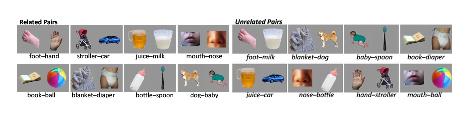
\includegraphics{images/fig1_wide.eps}
\caption{\label{fig:f-itempairs}Item-Pairs in Eyetracking Study. Infants
saw each image-pair twice. There were 16 trials in each trial-type
(related, unrelated), 32 trials total}
\end{figure}

\subsection*{Lab Visit Procedure}\label{labvisproc}
\addcontentsline{toc}{subsection}{Lab Visit Procedure}

First, staff explained the study to families and obtained consent for
either the yearlong study (including home recordings) or one-time
eyetracking, as relevant (approved by the U.Rochester IRB). Parents then
completed surveys about their child; see SI.

Next, the parent sat with the infant in their lap in a dimly lit testing
room, in front of an Eyelink 1000+ Eyetracker, which was in head-free
mode, and sampled monocularly at 500 Hz (\textless{}0.5\(^{\circ}\)
average accuracy; SR Research, Ontario, Canada). A small sticker on
infant's forehead tracked head movements. The experiment was run from a
computer that was back-to-back with the testing monitor, allowing for
adjustment if the child moved out of eyetracking range.

The experiment began with four ``warm-ups'', in which a single image was
labeled by a sentence played over speakers (e.g. ``Look at the apple!'')
Parents were then given a visor that blocked the screen (or closed their
eyes, n=3), and over-ear headphones. The experiment was also recorded by
camcorder to ensure compliance and monitor the child's state.

Next came 32 test trials, in which infants saw two images on a grey
background, and heard a sentence labeling one image; See
Fig.\ref{fig:f-itempairs}. An attention-getter was shown as needed. On
each test trial, parents spoke a single sentence aloud to their child,
which labeled one of the images on the screen; they first heard a
prerecorded sentence over headphones that they then repeated aloud (1).
Images were shown for 5s after target word onset; the length of time
before the parent said the target word after the images appeared varied
across trials, averaging \textasciitilde{}3--4s.

Each infant saw both trial-types (16 related and 16 unrelated trials,
interspersed pseudo-randomly). Infants were alternately assigned to two
trial orders, which counterbalanced side and ordering of images, target
items, and trial-type.

\subsubsection*{Stimuli}\label{stimuli}
\addcontentsline{toc}{subsubsection}{Stimuli}

16 common concrete nouns were chosen as target words based on corpora
and prior research, see SI and Fig.\ref{fig:f-itempairs}. Each word was
part of two item-pairs, one in each trial-type (related and unrelated,
e.g.~dog-baby and spoon-baby; n=16 item-pairs). Pairings maximized
semantic overlap within related pairs, and minimized it in unrelated
pairs. Semantic network analyses confirmed that related pairs were more
similar than unrelated pairs; see SI. Within trial-type, items were
paired to minimize phonetic overlap.\footnote{1 related pair unavoidably
  had the same initial consonant: book-ball.}

Audio stimuli were sentences recorded by a female using infant-directed
speech prosody in a sound-booth; they were 1.1-1.8s, normalized to 72db
(i.e.~a volume that allowed only parents to hear them when they were
played over the parent headphones). Infants only heard the sentences
from their parents (see Procedure). Each sentence occurred in 1 of 4
carrier phrases: ``Can you find the X?'', ``Where's the X?'', ``Do you
see the X?'', and ``Look at the X!'', where X is the target word (only 1
sentence frame was used per item-pair).

Visual stimuli were photos of each target and warm-up word, edited onto
a grey background, displayed at 500x500 pixels on a 27.4 by 34-cm LCD 96
PPI screen, at a viewing distance of 55-60cm. Warm-up images (n=4) were
displayed centrally. For test-trials (n=32), each image was centered
within the left and right half of the screen (counterbalanced across
trials). Each of 16 test photos occurred 4 times: once as target and as
distractor in each trial-type (related and unrelated; see
Fig.\ref{fig:f-itempairs}.).

\subsection*{Home Recording Procedure}\label{homerecproc}
\addcontentsline{toc}{subsection}{Home Recording Procedure}

Home recordings captured infants' typical environment through an
hour-long video recording, and, on a separate day, a daylong audio
recording. Before recording, parents were given a release form which
allowed up to 3 levels of sharing; see SI. Recordings that parents opted
to share with authorized researchers can be found on Databrary and
Homebank (n=43); access is available to researchers who complete ethics
certification and membership agreements through these repositories. See
sample clips in SI.

Video recordings took place at infants' homes. Research staff put a
specialized hat on the child, and a small Looxcie camera (8.4x1.7x1.3cm,
22g) was affixed above each ear with Velcro (one pointed slightly up and
one slightly down, to better capture the child's visual field). Staff
also put a camcorder on a tripod in the corner. Parents were given an
information sheet, asked to move the tripod if they changed rooms, and
given staff contacts. Staff left and returned after 1 hour.

At either the lab or home visit parents were given a LENA audio recorder
(8.6x5.6x1.3cm, 57g) and clothing with a LENA-pocket. (LENA Foundation,
Boulder, CO). Parents were asked to turn the recorder on when the child
awoke, and off at the end of the day or if they wanted to stop
recording. Recording time ranged from 10.66 to 16.00 hours (M=14.37).

\showmatmethods
\showacknow  \newline

\hypertarget{refs}{}
\hypertarget{ref-Bergelson2012}{}
1. Bergelson E, Swingley D (2012) At 6-9 months, human infants know the
meanings of many common nouns. \emph{Proceedings of the National Academy
of Sciences of the United States of America} 109(9):3253--8.

\hypertarget{ref-Bergelson2015b}{}
2. Bergelson E, Swingley D (2015) Early word comprehension in infants:
Replication and extension. \emph{Language Learning and Development}
11(4):369--380.

\hypertarget{ref-Parise2012}{}
3. Parise E, Csibra G (2012) Electrophysiological evidence for the
understanding of maternal speech by 9-month-old infants.
\emph{Psychological science} 23(7):728--33.

\hypertarget{ref-Tincoff1999}{}
4. Tincoff R, Jusczyk PW (1999) Some Beginnings of Word Comprehension in
6-Month-Olds. \emph{Psychological Science} 10(2):172--175.

\hypertarget{ref-Tincoff2012}{}
5. Tincoff R, Jusczyk PW (2012) Six-Month-Olds Comprehend Words That
Refer to Parts of the Body. \emph{Infancy} 17(4):432--444.

\hypertarget{ref-Gervain2010}{}
6. Gervain J, Mehler J (2010) Speech perception and language acquisition
in the first year of life. \emph{Annual review of psychology}
61:191--218.

\hypertarget{ref-Werker1984}{}
7. Werker JF, Tees RC (1984) Cross-language speech perception: Evidence
for perceptual reorganization during the first year of life.
\emph{Infant Behavior and Development} 7(1):49--63.

\hypertarget{ref-Polka1994}{}
8. Polka L, Werker JF (1994) Developmental changes in perception of
nonnative vowel contrasts. \emph{Journal of experimental psychology
Human perception and performance} 20:421--435.

\hypertarget{ref-Swingley2002b}{}
9. Swingley D, Aslin RN (2002) Lexical Neighborhoods and the Word-Form
representations of 14-Month-Olds. \emph{Psychological Science}
13(5):480--484.

\hypertarget{ref-Mani2010}{}
10. Mani N, Plunkett K (2010) Twelve-Month-Olds Know Their Cups From
Their Keps and Tups. \emph{Infancy} 15(5):445--470.

\hypertarget{ref-Vihman2004}{}
11. Vihman MM, Nakai S, DePaolis RA, Hallé PA (2004) The role of
accentual pattern in early lexical representation. \emph{Journal of
Memory and Language} 50(3):336--353.

\hypertarget{ref-Swingley2009a}{}
12. Swingley D (2009) Contributions of infant word learning to language
development. \emph{Philosophical transactions of the Royal Society of
London Series B, Biological sciences} 364(1536):3617--3632.

\hypertarget{ref-Bergelson2017a}{}
13. Bergelson E, Swingley D (2017) Young Infants' Word Comprehension
Given An Unfamiliar Talker or Altered Pronunciations. \emph{Child
Development}.
doi:\href{https://doi.org/10.1111/cdev.12888}{10.1111/cdev.12888}.

\hypertarget{ref-Smith2002}{}
14. Smith LB, Jones S, Landau B (2002) Object name learning provides
on-the-job training for attention. \emph{Psychological}. Available at:
\url{http://journals.sagepub.com/doi/abs/10.1111/1467-9280.00403}.

\hypertarget{ref-Wojcik2013a}{}
15. Wojcik EH, Saffran JR (2013) The ontogeny of lexical networks:
toddlers encode the relationships among referents when learning novel
words. \emph{Psychological science} 24(10):1898--1905.

\hypertarget{ref-Borovsky2016}{}
16. Borovsky A, Ellis E, Evans J, Elman J (2016) Semantic structure in
vocabulary knowledge interacts with lexical and sentence processing in
infancy. \emph{Child Development}. Available at:
\url{http://onlinelibrary.wiley.com/doi/10.1111/cdev.12554/full}.

\hypertarget{ref-Luche2014}{}
17. Luche CD, Durrant S, Floccia C, Plunkett K (2014) Implicit meaning
in 18-month-old toddlers. \emph{Developmental science}:1--8.

\hypertarget{ref-Arias-Trejo2010}{}
18. Arias-Trejo N, Plunkett K (2010) The effects of perceptual
similarity and category membership on early word-referent
identification. \emph{Journal of experimental child psychology}
105(1-2):63--80.

\hypertarget{ref-Bergelson2017}{}
19. Bergelson E, Aslin R (2017) Semantic Specificity in One-Year-Olds'
Word Comprehension. \emph{Language Learning and Development}.
doi:\href{https://doi.org/10.1080/15475441.2017.1324308}{10.1080/15475441.2017.1324308}.

\hypertarget{ref-Neely1991}{}
20. Neely JH (1991) Semantic priming effects in visual word recognition:
a selective review of current findings and theories. \emph{Basic
Processes in Reading: Visual Word Recognition}, eds Besner D, Humphreys
G (Lawrence Erlbaum Associates, Hillsdale), pp 264--336.

\hypertarget{ref-Huettig2005}{}
21. Huettig F, Altmann GTM (2005) Word meaning and the control of eye
fixation: Semantic competitor effects and the visual world paradigm.
\emph{Cognition} 96(1):23--32.

\hypertarget{ref-Dahan2005}{}
22. Dahan D, Tanenhaus MK (2005) Looking at the rope when looking for
the snake: conceptually mediated eye movements during spoken-word
recognition. \emph{Psychonomic bulletin \& review} 12(3):453--459.

\hypertarget{ref-Hart1992}{}
23. Hart B, Risley TR (1992) American parenting of language-learning
children: Persisting differences in family-child interactions observed
in natural home environments. \emph{Developmental Psychology}
28(6):1096--1105.

\hypertarget{ref-Weisleder2013}{}
24. Weisleder A, Fernald A (2013) Talking to children matters: early
language experience strengthens processing and builds vocabulary.
\emph{Psychological science} 24(11):2143--2152.

\hypertarget{ref-Hoff2002}{}
25. Hoff E, Naigles LG (2002) How children use input to acquire a
lexicon. \emph{Child development} 73(2):418--433.

\hypertarget{ref-Shneidman2012}{}
26. Shneidman L, Goldin‐Meadow S (2012) Language input and acquisition
in a Mayan village: how important is directed speech?
\emph{Developmental science}. Available at:
\url{http://onlinelibrary.wiley.com/doi/10.1111/j.1467-7687.2012.01168.x/full}.

\hypertarget{ref-Lieven1994}{}
27. Lieven E (1994) Crosslinguistic and crosscultural aspects of
language addressed to children. Available at:
\url{http://psycnet.apa.org/psycinfo/1994-98392-003}.

\hypertarget{ref-Debaryshe1993}{}
28. Debaryshe BD (1993) Joint picture-book reading correlates of early
oral language skill. \emph{Journal of child language} 20(2):455--461.

\hypertarget{ref-Montag2015}{}
29. Montag JL, Jones MN, Smith LB (2015) The Words Children Hear:
Picture Books and the Statistics for Language Learning.
\emph{Psychological Science} 26(9):1489--1496.

\hypertarget{ref-Rost2009}{}
30. Rost GC, McMurray B (2009) Speaker variability augments phonological
processing in early word learning. \emph{Developmental Science}
12(2):339--349.

\hypertarget{ref-Brent2001}{}
31. Brent MR, Siskind JM (2001) The role of exposure to isolated words
in early vocabulary development. \emph{Cognition} 81(2):B33-----B44.

\hypertarget{ref-Seidl2006}{}
32. Seidl A, Johnson EK (2006) Infant word segmentation revisited: Edge
alignment facilitates target extraction. \emph{Developmental Science}
9(6):565--573.

\hypertarget{ref-Medina2011}{}
33. Medina TN, Snedeker J, Trueswell JC, Gleitman LR (2011) How words
can and cannot be learned by observation. \emph{Proceedings of the
National Academy of Sciences of the United States of America}
108:9014--9019.

\hypertarget{ref-Yurovsky2013}{}
34. Yurovsky D, Smith LB, Yu C (2013) Statistical word learning at
scale: the baby's view is better. \emph{Developmental science}
16(6):959--966.

\hypertarget{ref-McGillion2013}{}
35. McGillion ML, et al. (2013) Supporting Early Vocabulary Development:
What Sort of Responsiveness Matters? \emph{IEEE Transactions on
Autonomous Mental Development} 5(3):240--248.

\hypertarget{ref-Bergelson2013}{}
36. Bergelson E, Swingley D (2013) The acquisition of abstract words by
young infants. \emph{Cognition} 127(3):391--7.

\hypertarget{ref-MacWhinney2000}{}
37. MacWhinney B (2000) \emph{The CHILDES Project: Tools for Analyzing
Talk, Volume II: The database} (Lawrence Erlbaum, Mahwah, NJ). 3rd Ed.

\hypertarget{ref-Dale1996}{}
38. Dale PS, Fenson L (1996) Lexical development norms for young
children. \emph{Behavior Research Methods, Instruments, \{\&\}
Computers} 28(1):125--127.

\hypertarget{ref-Libertus2013}{}
39. Libertus K, Landa RJ (2013) The Early Motor Questionnaire (EMQ): A
parental report measure of early motor development. \emph{Infant
Behavior and Development} 36:833--842.

\hypertarget{ref-Walle2014}{}
40. Walle EA, Campos JJ (2014) Infant language development is related to
the acquisition of walking. \emph{Developmental Psychology}
50(2):336--348.



% Bibliography
% \bibliography{pnas-sample}

\end{document}

